% !Mode:: "TeX:UTF-8"
%!TEX program  = xelatex

%\documentclass{cumcmthesis}
\documentclass[withoutpreface,bwprint]{cumcmthesis} %去掉封面与编号页


\title{全国大学生数学建模竞赛编写的 \LaTeX{} 模板}
\tihao{A}
\baominghao{2017000}
\schoolname{长江大学}
\membera{刘艳}
\memberb{朱艳玲}
\memberc{孔庆亮}
\supervisor{数模指导组}
\yearinput{2017}
\monthinput{08}
\dayinput{11}

\begin{document}

 \maketitle
 \begin{abstract}


\keywords{太阳高度角\quad  曲线拟合\quad   非线性优化模型\quad  受力分析}
\end{abstract}

\section{问题重述} 

随着现代社会科技水平的不断提高和通信技术的愈加完善,定位技术受到了越来越多的关注。太阳影子定位技术就是通过分析视频中物体的太阳影子变化,确定视频拍摄的地点和日期的一种方法。根据附件,解决以下问题:
\item 建立影子长度变化的数学模型,分析影子长度关于各个参数的变化规律,并应用你们建立的模型画出2015年10月22日北京时间9:00-15:00之间天安门广场(北纬39度54分26秒,东经116度23分29秒)3米高的直杆的太阳影子长度的变化曲线。
\item 根据某固定直杆在水平地面上的太阳影子顶点坐标数据,建立数学模型确定直杆所处的地点。将你们的模型应用于附件1的影子顶点坐标数据,给出若干个可能的地点。
\item 根据某固定直杆在水平地面上的太阳影子顶点坐标数据,建立数学模型确定直杆所处的地点和日期。将你们的模型分别应用于附件2和附件3的影子顶点坐标数据,给出若干个可能的地点与日期。
\item 附件4为一根直杆在太阳下的影子变化的视频,并且已通过某种方式估计出直杆的高度为2米。请建立确定视频拍摄地点的数学模型,并应用你们的模型给出若干个可能的拍摄地点。
如果拍摄日期未知,你能否根据视频确定出拍摄地点与日期?


\subsection{问题的提出}



\section{模型的假设}

\begin{itemize}
\item 地球为均匀球体;
\item 忽略大气折射作用,即太阳光线平行照射地球;
\item 钢筋强度足够大,不弯曲;
\item 假设地面平整。
\end{itemize}

\section{符号说明}

\begin{table}[!htbp]
    \centering
    \begin{tabular}{cl}
        \toprule
        \multicolumn{2}{c}{\large 模型记号说明}\\
        \midrule
        h	        & 太阳高度角 \\
        \phi	    & 观测地地理纬度  \\
        \delta	    & 太阳赤纬角  \\
        t	        & 地方时(时角) \\  
        A	        & 太阳方位角 \\
        H          & 直杆长度  \\
        l          & 影子长度  \\

    \end{tabular}
\end{center}
 
\section{问题分析}

\subsection{问题一分析}
对于问题一,我们已知直杆的长度为 米高,根据物理光学的知识,如果我们再知道平行光源的入射角,就可以知道影子的长度。但实际情况是,由于太阳光线的入射角(高度角)是随时间变化的,也导致影子的长度随时间变化,这样就可以转化为影子的长度随时间的变化规律。

 
 

% 问题流程图:
% \begin{figure}[!h]
% \centering
% 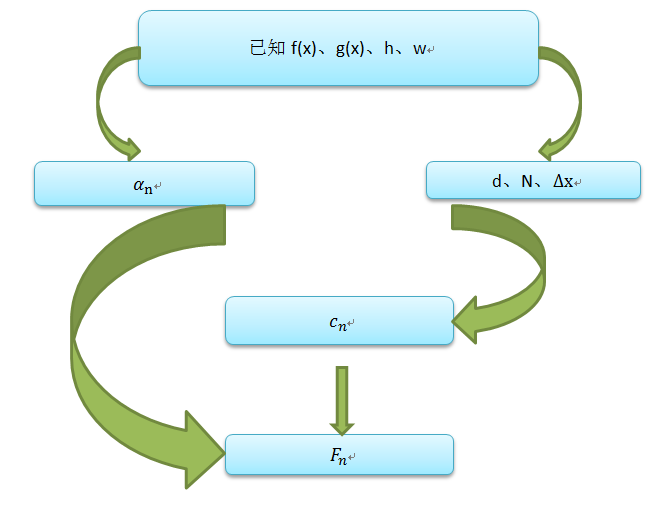
\includegraphics[width=.6\textwidth]{1.png}
% \caption{问题三流程图}
% \end{figure}

% \section{绘制普通三线表格}
% 表格应具有三线表格式,因此常用 booktabs宏包,其标准格式如表~\ref{tab001}~所示。
% \begin{table}[!htbp]
% \caption{标准三线表格}\label{tab001} \centering
% \begin{tabular}{ccccc}
% \toprule[1.5pt]
% $D$(in) & $P_u$(lbs) & $u_u$(in) & $\beta$ & $G_f$(psi.in)\\
% \midrule[1pt]
%  5 & 269.8 & 0.000674 & 1.79 & 0.04089\\
% 10 & 421.0 & 0.001035 & 3.59 & 0.04089\\
% 20 & 640.2 & 0.001565 & 7.18 & 0.04089\\
% \bottomrule[1.5pt]
% \end{tabular}
% \end{table}

% 其绘制表格的代码及其说明如下。
% \begin{tcode}
% \begin{table}[!htbp]
% \caption[标签名]{中文标题}
% \begin{tabular}{cc...c}
% \toprule[1.5pt]
% 表头第1个格   & 表头第2个格   & ... & 表头第n个格  \\
% \midrule[1pt]
% 表中数据(1,1) & 表中数据(1,2) & ... & 表中数据(1,n)\\
% 表中数据(2,1) & 表中数据(2,2) & ... & 表中数据(2,n)\\
% ...................................................\\
% 表中数据(m,1) & 表中数据(m,2) & ... & 表中数据(m,n)\\
% \bottomrule[1.5pt]
% \end{tabular}
% \end{table}
% \end{tcode}

% \bigskip
% table环境是一个将表格嵌入文本的浮动环境。
% tabular环境的必选参数由每列对应一个格式字符所组成:c表示居中,l表示左对齐,r表示右对齐,其总
% 个数应与表的列数相同。此外,\verb|@{文本}|可以出现在任意两个上述的列格式之间,其中的文本将被插入每一行
% 的同一位置。表格的各行以\verb|\\|分隔,同一行的各列则以\&分隔。
% \verb|\toprule|、\verb|\midrule|和\verb|\bottomrule|三个命令是由booktabs宏包提供的,其
% 中\verb|\toprule|和\verb|\bottomrule|分别用来绘制表格的第一条(表格最顶部)和第三条(表格最底部)水平线,
% \verb|\midrule|用来绘制第二条(表头之下)水平线,且第一条和第三条水平线的线宽为1.5pt,第二条水平线的线宽为1pt。
% 引用方法:“如表~\verb|\ref{标签名}|~所示”。


%参考文献
\begin{thebibliography}{9}%宽度9
 \bibitem{bib:one} ....
 \bibitem{bib:two} ....
\end{thebibliography}


\newpage
%附录
\appendix

\section{matlab 源程序}
\subsection{太阳高度角}

\begin{lstlisting}[language=matlab]
function data = angle(latitude,longitude,month,day,start_time,end_time)   % latitude纬度  longitude经度
%% 求解太阳高度角
%   h太阳高度角 phi纬度 delt赤纬角 t时角
%   $ sin(h) = sin(phi)sin(delta)+cos(phi)cos(delta)cos(t) $

phi = latitude;

%% 求赤纬角

delta = -(23+27/60)*(29/90);

%% 求时角
hours = start_time:0.0001:end_time;
t = 15 .* (hours - 12)*(pi/180) + (longitude - 120)*(pi/180);

%% 太阳高度角
data = abs(asin(sin(phi).*sin(delta) + cos(phi).*cos(delta).*cos(t)));

\end{lstlisting}

\subsection{问题一影长变化}
\begin{lstlisting}[language=matlab]

%   求影长
clc,clear

%% 输入参数
H = 3;
latitude = 39+54./60+26+(60.*60);
longitude = 116+23./60+29/(60.*60);
month = 10;
day = 22;
start_time = 9.0;
end_time = 15.0;

%% 求解影长
h = angle(latitude,longitude,month,day,start_time,end_time);  % latitude纬度  longitude经度
L = H ./ tan(h);

%% 寻找最短影长和时间
shortL = 10;
for j = 1:length(L)
    shortL = min(shortL,L(j));
    if min(shortL,L(j)) == L(j)
        time_shortL = j;
    end
end
hour_time_shortL = 9 + floor(time_shortL / 10000);
minute_time_shortL = 60*(time_shortL - floor(time_shortL / 10000)*10000)/10000;

%% 画图
figure
plot(start_time:0.0001:end_time,L,'b-');
hold on;
title('3米高的直杆的太阳影子长度的变化曲线');
xlabel('时刻');
ylabel('直杆的太阳影子长度');
j = 9 + time_shortL/10000 * ones(1,121);
line = 4:0.01:5.2;
plot(j,line,'r-');
hold on;
legend('影子长度的变化曲线','最短影子时间点:12:14:44');


\end{lstlisting}

% \section{规划解决程序--lingo源代码}
% \begin{lstlisting}[language=c]
% kk=2;
% [mdd,ndd]=size(dd);
% while ~isempty(V)
%     [tmpd,j]=min(W(i,V));tmpj=V(j);
% for k=2:ndd
%     [tmp1,jj]=min(dd(1,k)+W(dd(2,k),V));
%     tmp2=V(jj);tt(k-1,:)=[tmp1,tmp2,jj];
% end
%     tmp=[tmpd,tmpj,j;tt];[tmp3,tmp4]=min(tmp(:,1));
% if tmp3==tmpd, ss(1:2,kk)=[i;tmp(tmp4,2)];
% else,tmp5=find(ss(:,tmp4)~=0);tmp6=length(tmp5);
% if dd(2,tmp4)==ss(tmp6,tmp4)
%     ss(1:tmp6+1,kk)=[ss(tmp5,tmp4);tmp(tmp4,2)];
% else, ss(1:3,kk)=[i;dd(2,tmp4);tmp(tmp4,2)];
% end;
% end
%     dd=[dd,[tmp3;tmp(tmp4,2)]];V(tmp(tmp4,3))=[];
%     [mdd,ndd]=size(dd);
%     kk=kk+1;
% end;
% S=ss;
% D=dd(1,:);
% \end{lstlisting}


\end{document} 
